\chapter{Theoretical background}
\label{chap:refs}

\section{Glossary}

\begin{tabular}{p{0.22\linewidth}p{0.7\linewidth}}
    SDN & Software-defined networking. Additional details can be found in \cref{sec:sdn}. \\ % <--

    OVS & Open vSwitch (\url{https://www.openvswitch.org/}). Details in \cref{sec:ovs}. \\ % <--

    OVN & Open Virtual Network (\url{https://docs.ovn.org/en/latest/}). Details in \cref{sec:ovn}. \\ % <--

    CNI & Container network interface \cite{CNI}. Specification for writing networking plugins for Kubernetes. The plugin handles assigning IP addresses and routing packets across the cluster. \\

    OVN-Kubernetes & CNI plugin using OVN (\cref{sec:ovnkube}). \\

    Forwarding tables & Network switches use forwarding tables to decide where to forward a received packet. In Ethernet switches, the forwarding tables consist of MAC address to network port mapping. SDNs generalized forwarding tables so that they can match packets in any way deemed useful, most commonly on any header values from the second, third, and fourth layers of the OSI model. \\

    OpenFlow & Network configuration protocol used between an SDN controller and SDN switches. OpenFlow allows remote configuration of forwarding tables in network switches. Details in \cref{sec:openflow} \\

    RTT & round-trip time  \\

\end{tabular}

\section{Software-defined networking (SDN)}
\label{sec:sdn}


\begin{figure}
    \centering
    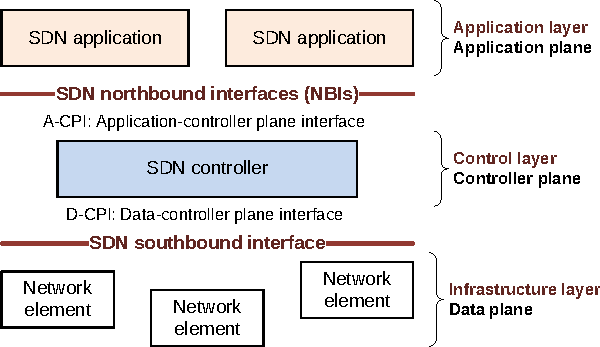
\includegraphics[width=.6\linewidth]{img/sdn_basic_schema.pdf}
    \caption{A schema of basic SDN components (originally from \cite{SdnArch}).}
    \label{fig:sdn-schema}
\end{figure}

\emph{Software-defined networking} is a loosely defined concept of separating the networking data plane (infrastructure layer) and the control plane (control layer) into separate components. In traditional networking architectures, each network device makes forwarding and/or routing decisions fully autonomously. SDNs separate the decision-making and data processing into distinct layers (see \cref{fig:sdn-schema}) and define two main interfaces. \emph{SDN applications} provide the \emph{SDN controller} with networking requirements using the \emph{northbound interface}. The controller then configures the actual network equipment using the \emph{southbound interface}.

\section{OpenFlow}
\label{sec:openflow}

% \footnote{\url{https://opennetworking.org/sdn-resources/openflow-switch-specification/}}
\emph{OpenFlow} \cite{OFSpec} is a protocol for configuring packet forwarders (generalized switches). OpenFlow is the de-facto standard protocol for the southbound interface in an SDN.

In OpenFlow, there are multiple forwarding tables for every network switch. Every table is identified with a number and contains a set of rules with priorities. Each rule consists of matching criteria, usage statistics and actions. The following is an example of an OpenFlow rule dumped from a running Open vSwitch using the \ident{ovs-ofctl dump-flows \$BRIDGE} command:

\begin{verbatim}
cookie=0x802cec73, duration=22932.301s, table=33, n_packets=0,
n_bytes=0, priority=75,
arp,metadata=0x7,dl_src=24:6e:96:3c:4c:5c,arp_op=1
actions=load:0x8004->NXM_NX_REG15[],resubmit(,37)
\end{verbatim}

The third line in the example specifies the rule criteria. Generally, the matching criteria can include masks for header values from Ethernet, IP, transport layer protocols (TCP, UDP, ...), and more depending on the exact version of the OpenFlow protocol. The criteria can check for an exact value match or with a wildcard.

The action in a flow rule can forward the packet to a port, change a value of a header field, store an arbitrary value as metadata accompanying the packet in further processing, resubmit the packet to a different table and more. For the complete list of actions, see the OpenFlow specification \cite{OFSpec} or the \ident{ovs-actions} manpage \cite{OVSActionsMan}.

In addition to the externally configured flow rules, the forwarding tables also contain statistics updated every time the flow rule is used. The OpenFlow controller can then query switches for these statistics.

\section{Open vSwitch}
\label{sec:ovs}

\emph{Open vSwitch} (OVS) \cite{OVSWeb} \cite{OVSSource} \cite{KernelSource} is a multilayer virtual switch. OVS runs as a software switch on all major platforms and supports hardware offload for its data processing layers. The supported OpenFlow protocol allows any SDNs to use OVS in its infrastructure layer.

The internal architecture of OVS mirrors the SDN architecture (see \cref{fig:ovs-arch-schema}) with a control plane and data plane. \ident{ovs-vswitchd} is the OVS's control process. \ident{ovs-vswitchd} communicates via the OpenFlow protocol and stores the configured flow rules in a purpose-built Open vSwitch Database (OVSDB). Alternatively, the database can be accessed externally, and OVS can be configured without using the OpenFlow wire protocol.

A \emph{datapath} is the primary part of OVS's data layer, the lowest component of OVS physically forwarding packets between configured ports. There are multiple datapath implementations, some of them implemented fully in the \ident{ovs-vswitchd} process, some of them using extra kernel modules for improved performance. \ident{ovs-vswitchd} translates the OpenFlow flow rules into a more efficient and simplified form. These simplified flow rules are then used by the datapaths to make forwarding decisions. We discuss datapath internals in more detail in \cref{sec:ovs-datapath}.

\begin{table}[h!]
    \begin{center}
        \caption{Overview of OVS components}
        \label{tab:ovs-components}
        \begin{tabular}{p{0.2\linewidth}|p{0.7\linewidth}}
            \textbf{Component} & \textbf{Description} \\
            \hline
            \ident{ovsdb} & OVSDB instance storing the OpenFlow flow rules \\
            \hline
            \ident{ovs-vswitchd} & a process managing datapaths and providing OpenFlow configuration interface \\
            \hline
            datapath & a logical component in \ident{ovs-vswitchd}, does the actual packet forwarding \\
        \end{tabular}
    \end{center}
\end{table}


% \tablefootnote{\url{https://docs.openvswitch.org/en/latest/ref/ovsdb.7/}}
% \tablefootnote{\url{http://www.openvswitch.org/support/dist-docs/ovs-vswitchd.8.html}}

\section{Open Virtual Network}
\label{sec:ovn}

\emph{Open Virtual Network} (OVN) \cite{OpenStackOVNDocs} \cite{OVNSource} is an SDN combining Open vSwitch with network tunnels (by default GENEVE) for its infrastructure layer. Applications communicate with OVN through the \ident{northdb}, an OVSDB instance storing high-level network configuration in terms of traditional networking concepts. The \ident{ovn-northd} process translates the configuration into logical datapath flows and stores the result in the \ident{southdb} OVSDB instance. The \ident{ovn-controller} then distributes the flows from the \ident{southdb} into individual OVS databases.

\begin{table}[h!]
    \begin{center}
        \caption{Overview of OVN components}
        \label{tab:ovn-components}
        \begin{tabular}{p{0.23\linewidth}|p{0.47\linewidth}|p{0.2\linewidth}}
            \textbf{Component} & \textbf{Description} & \textbf{How it runs} \\
            \hline
            \ident{northdb} & OVSDB instance storing network configuration in terms of traditional networking concepts & centralized or distributed \\
            \hline
            \ident{ovn-northd} & process translating configuration into logical flows & centralized or distributed \\
            \hline
            \ident{southdb} & OVSDB instance storing network configuration in terms of logical flows & centralized or distributed\\
            \hline
            \ident{ovn-controller} & configures local OVS from the \ident{southdb} & locally on every node\\
        \end{tabular}
    \end{center}
\end{table}


\section{OVN-Kubernetes}
\label{sec:ovnkube}

\emph{OVN-Kubernetes} \cite{OVNKubeSource} is a Kubernetes CNI plugin using OVN in the background. OVN-Kubernetes configures OVN and OVS on all cluster nodes and translates network reconfiguration requests from the CNI API into configuration changes for OVN.

\section{Open vSwitch Datapaths}
\label{sec:ovs-datapath}

\begin{figure}
    \centering
    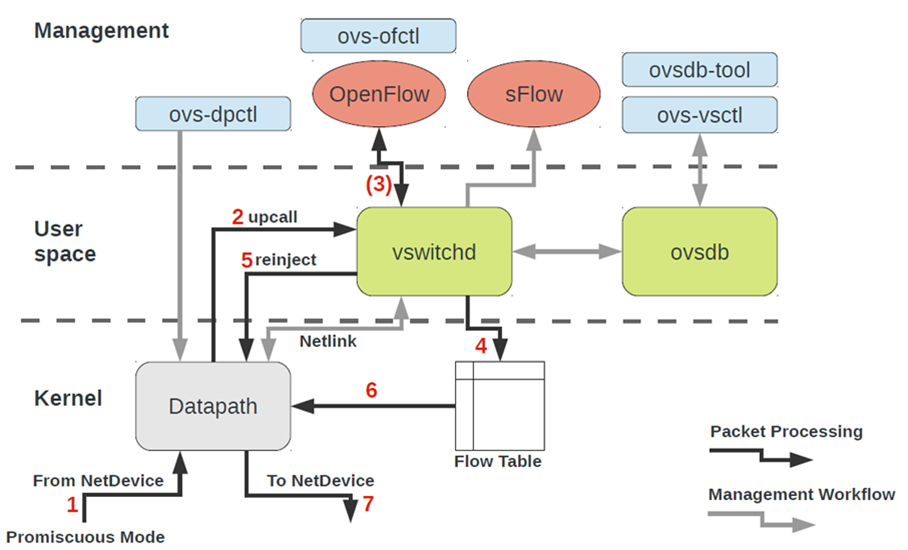
\includegraphics[width=.9\linewidth]{img/ovs_architecture_01.png}
    \caption{Schema of OVS internal architecture (originally from \cite{OVSArchImage}).}
    \label{fig:ovs-arch-schema}
\end{figure}

OVS processes packets in \href{https://github.com/openvswitch/ovs/blob/e90a0727f17f6ad915a32735a8c0b282f2c8cd6f/lib/dpif.h}{datapaths}\footnote{digital version of this text contains hyperlinks to the relevant source code}. All datapaths implement a common \href{https://github.com/openvswitch/ovs/blob/e90a0727f17f6ad915a32735a8c0b282f2c8cd6f/lib/dpif-provider.h\#L107-L117}{interface} hiding the implementation details of low-level packet processing from the layers above.

The two most commonly used datapath implementations are \href{https://github.com/openvswitch/ovs/blob/e90a0727f17f6ad915a32735a8c0b282f2c8cd6f/lib/dpif-netdev.c}{\ident{netdev}} and \href{https://github.com/openvswitch/ovs/blob/e90a0727f17f6ad915a32735a8c0b282f2c8cd6f/lib/dpif-netlink.c}{\ident{netlink}}. They are named after the mechanism used for integrating with the operating system. The \ident{netlink} datapath is Linux-specific and uses a special kernel module. The \ident{netdev} datapath is implemented in userspace.

Datapaths are optimized for high-performance packet processing and they completely handle most of the packets that come through them. Consequently, the forwarding tables in the datapaths are not equivalent to the OpenFlow forwarding tables and a translation mechanism between the two forwarding table formats is present. The translation is performed lazily. When a packet does not match any rule in the datapath forwarding table, an \emph{upcall} is made and the packet is passed out of the datapath into the upper layers of \ident{ovs-vswitchd}. \ident{ovs-vswitchd} performs a full lookup through the OpenFlow forwarding tables and generates a new datapath flow rule which gets inserted into the datapath together with the packet itself.

We use the name \emph{fast path} to refer to datapath-only packet processing. If the packet misses all datapath flow rules and generates an upcall, we say that it took the \emph{slow path}.

\paragraph{The \ident{netdev} datapath}
The \ident{netdev} datapath is a multiplatform datapath implementation entirely in user space. All major operating systems are currently supported.

The netdev datapath supports various configurations according to the system it is running on. The most basic deployment is rather slow as all packets have to cross the userspace boundary twice. However, the datapath can be configured with several types of accelerators significantly lowering the packet processing cost. The datapath can be accelerated using DPDK \cite{DPDK}, AF\_XDP sockets \cite{XDP} or offloaded to hardware using TC \cite{TCOffload}.

Our research does not target the \ident{netdev} datapath.

\paragraph{The \ident{netlink} datapath}
The \ident{netlink} datapath is Linux-specific. It resides partially in a kernel module and partially in user space. The kernel module does most of the packet processing. The userspace communicates with the kernel over a netlink socket, hence the name. Only the slow path passes data from the kernel space to the user space.

Our research is focused on the \ident{netlink} datapath as it is the most commonly deployed datapath in Kubernetes clusters. Unless stated otherwise, the rest of the thesis always assumes the context of the \ident{netlink} datapath.

\subsection{Interactions between the fast path and the slow path}

Packets always start their journey in the kernel. They enter the \ident{openvswitch} module where they are checked against a set of flow rules stored in the flow table (OVS's forwarding table). If a flow rule matches the packet, its actions are executed. Otherwise, the packet is sent to the user space.

\begin{verbatim}
def process_packet_in_kernel(packet):
    for flow_rule in flow_table:
        if flow_rule criteria match the packet:
            execute the flow_rule actions
            return
    
    make an upcall to the user space
\end{verbatim}

The slow path gets involved when the fast path fails (no flow rule match) or when the action in the flow rule explicitly asks for it. The packet is sent to the user space via a netlink socket in an upcall. \ident{ovs-vswitchd} receives the packet, processes it according to the OpenFlow rules and reinjects it back into the kernel. Additionally, a new flow rule might be generated and installed into the kernel to speed up the future processing of similar packets.

The packets in the fast path are not buffered and they are processed immediately. The slow-path buffers packets when they are passed from kernel to user space, introducing additional latency.

\subsection{The fast-path}
\label{the-fast-path}

\subsubsection{The data structures}
\label{the-data-structures}

The flow table (\href{https://elixir.bootlin.com/linux/v6.2.6/source/net/openvswitch/flow_table.h\#L62}{\ident{struct\ flow\_table}}) is an in-kernel data structure, which stores flows rules (\href{https://elixir.bootlin.com/linux/v6.2.6/source/net/openvswitch/flow.h\#L221}{\ident{struct\ sw\_flow}}) and allows for fast matching with individual packets. Similar to OpenFlow flow rules, every datapath flow contains a list of actions (\href{https://elixir.bootlin.com/linux/v6.2.6/source/net/openvswitch/flow.h\#L206}{\ident{struct\ sw\_flow\_actions}}), statistics (\href{https://elixir.bootlin.com/linux/v6.2.6/source/net/openvswitch/flow.h\#L213}{\ident{struct sw\_flow\_stats}}), a flow key (\href{https://elixir.bootlin.com/linux/v6.2.6/source/net/openvswitch/flow.h\#L75}{\ident{struct\ sw\_flow\_key}}) and a flow mask (\href{https://elixir.bootlin.com/linux/v6.2.6/source/net/openvswitch/flow.h\#L183}{\ident{struct\ sw\_flow\_mask}}).

The flow key and the flow mask are the matching criteria. The combination of both of these enables fast matching with the possibility of wildcards. The key is a complex structure with parsed-out packet header values. It can be created from any packet with the function \href{https://elixir.bootlin.com/linux/v6.2.6/source/net/openvswitch/flow.c\#L886}{\ident{key\_extract()}}. The mask specifies which bits are significant when comparing two keys.

\begin{verbatim}
def equals(key1, key2, mask) -> bool:
    return (key1 & mask) == (key2 & mask)
\end{verbatim}


\subsubsection{The matching algorithm}
\label{subsec:matching-algo}

When the kernel processes a packet, it creates the packet's corresponding flow key and looks for matching flows in the flow table. The packet can match any number of flows, but only the first matching rule is always used. The userspace component is responsible for preventing overlapping conflicting flow rules.

The flow table stores the flows in a hash table. The lookup key is the masked \ident{sw\_flow\_key}. Therefore, to find a flow for a packet, the kernel has to try several masks. The lookup procedure could look like this:

\begin{verbatim}
def lookup(flow_table, key):
    for mask in flow_table.mask_array:
        masked_key = apply mask to key
        if masked_key in flow_table.flows:
            return flow_table.flows[masked_key]
    return None
\end{verbatim}
    

The real implementation (\href{https://elixir.bootlin.com/linux/v6.2.5/source/net/openvswitch/flow_table.c\#L785}{\ident{ovs\_flow\_tbl\_lookup\_stats}}) is in principle similar, but more optimized:

\begin{enumerate}
\def\labelenumi{\arabic{enumi}.}
\item
  The kernel keeps mask usage statistics and the \ident{mask\_array} is
  kept sorted with the most used masks first
  (\href{https://elixir.bootlin.com/linux/v6.2.5/source/net/openvswitch/flow_table.c\#L1107}{\ident{ovs\_flow\_masks\_rebalance()}}).
  This happens
  \href{https://elixir.bootlin.com/linux/v6.2.5/source/net/openvswitch/datapath.c\#L2536}{periodically}
  based on a time interval.
\item
  There is already a \ident{sk\_buff}\footnote{a kernel structure wrapping all packets}
  \href{https://elixir.bootlin.com/linux/v6.2.5/source/include/linux/skbuff.h\#L1537}{hash}
  based on source/destination addresses and ports. The lookup procedure
  makes use of the hash by having a fixed size
  (\href{https://elixir.bootlin.com/linux/v6.2.5/source/net/openvswitch/flow_table.c\#L41}{256})
  hash table storing references to their masks. The cached masks are
  then tried first. If there is no match, a standard lookup over all masks
  follows and the cache entry \href{https://elixir.bootlin.com/linux/v6.2.5/source/net/openvswitch/flow_table.c\#L842}{is replaced} with a new flow. This helps with burst performance.
\end{enumerate}

\subsection{The actions}
\label{subsec:ovs-actions}

The actions in a flow rule are similar to actions in OpenFlow. They are described in the \href{https://www.man7.org/linux/man-pages/man7/ovs-actions.7.html}{manpages \ident{ovs-actions(7)}}.

Special attention should be given to the recirculation action, which corresponds to the \ident{resubmit} OpenFlow action. This action resubmits the packet to the datapath again, updating its flow key's \ident{recirc\_id} to a new value. This effectively simulates having multiple flow tables in the datapath with only a single physical table.

% https://andreaskaris.github.io/blog/networking/ovs_recirculation/

\subsection{The slow-path}

The user space process (\href{https://www.man7.org/linux/man-pages/man8/ovs-vswitchd.8.html}{\ident{ovs-vswitchd}}) communicates with the kernel over a netlink socket. When a packet leaves the
fast-path, it is temporarily buffered in a queue (\href{https://elixir.bootlin.com/linux/v6.2.6/source/net/openvswitch/datapath.c\#L311}{\ident{ovs\_dp\_upcall()}}) when crossing the kernel boundary.

\ident{ovs-vswitchd} reads packets from the kernel in several \emph{handler threads}. The datapath interface defines a \href{https://github.com/openvswitch/ovs/blob/e90a0727f17f6ad915a32735a8c0b282f2c8cd6f/lib/dpif-provider.h\#L387-L408}{\ident{recv()}} function for receiving a single packet from the kernel. The netlink datapath implements it with the \href{https://github.com/openvswitch/ovs/blob/e90a0727f17f6ad915a32735a8c0b282f2c8cd6f/lib/dpif-netlink.c\#L3132-L3134}{\ident{dpif\_netlink\_recv()}} function.

Higher up, the \ident{recv()} datapath interface function is used in a generic \href{https://github.com/openvswitch/ovs/blob/e90a0727f17f6ad915a32735a8c0b282f2c8cd6f/lib/dpif.c\#L1591-L1611}{\ident{dpif\_recv()}} function which also provides an useful \href{https://github.com/openvswitch/ovs/blob/e90a0727f17f6ad915a32735a8c0b282f2c8cd6f/lib/dpif.c\#L1618}{tracepoint} for measurements. Even higher up the abstraction stack, the \href{https://github.com/openvswitch/ovs/blob/e90a0727f17f6ad915a32735a8c0b282f2c8cd6f/ofproto/ofproto-dpif-upcall.c\#L829-L830}{\ident{recv\_upcalls()}} function in the file \ident{ofproto-dpif-upcall.c} reads packets in batches, which are then processed by \href{https://github.com/openvswitch/ovs/blob/e90a0727f17f6ad915a32735a8c0b282f2c8cd6f/ofproto/ofproto-dpif-upcall.c\#L1639-L1641}{\ident{handle\_upcalls()}}. The \ident{handle\_upcalls()} function essentially transforms the list of packets into a list of operations that should be executed on the datapath. This includes adding new flows to the datapath as well as simply sending packets where they belong.

\subsection{Additional \ident{ovs-vswitchd} tasks}
\label{subsec:ovs-tasks}

Parallel with upcall processing in the handler threads, OVS also runs several maintenance tasks:
\begin{itemize}
    \item A \href{https://github.com/openvswitch/ovs/blob/e90a0727f17f6ad915a32735a8c0b282f2c8cd6f/ofproto/ofproto-dpif-upcall.c\#L3312-L3336}{balancing task} makes sure that when the system is under stress, the most frequently used flow rules are in the kernel.
    \item \href{https://github.com/openvswitch/ovs/blob/e90a0727f17f6ad915a32735a8c0b282f2c8cd6f/ofproto/ofproto-dpif-upcall.c\#L83-L111}{The revalidator threads} periodically dump statistics from the kernel and remove old unused flows. The number of revalidator threads scales with the number of available cores on the system.
\end{itemize}

% TODO add sources
%
% \begin{center}\rule{0.5\linewidth}{0.5pt}\end{center}
% 
% \hypertarget{sources}{%
% \section{Sources}\label{sources}}
% 
% \begin{itemize}
% \tightlist
% \item
%   \href{https://docs.openvswitch.org/en/latest/contents/}{Open vSwitch
%   online documentation}
% 
%   \begin{itemize}
%   \tightlist
%   \item
%     \href{https://docs.openvswitch.org/en/latest/topics/datapath/}{Open
%     vSwitch Datapath Development Guide}
%   \end{itemize}
% \item
%   \href{https://elixir.bootlin.com/linux/v6.2.6/source}{Linux Kernel
%   source code}
% \item
%   \href{https://github.com/openvswitch/ovs/tree/51778134d4c8a84801230b1e5a7d59e180d9e8b5}{Open
%   vSwitch source code}
% \item
%   \href{https://developers.redhat.com/articles/2022/02/07/investigating-cost-open-vswitch-upcalls-linux}{RedHat
%   Developer Blog: Investigating the cost of Open vSwitch upcalls in
%   Linux}
% \item
%   \href{https://hustcat.github.io/an-introduction-to-ovs-architecture/}{An
%   introduction to OVS architecture}
% \end{itemize}